\documentclass{beamer}
\usepackage{geometry}
\usepackage{graphicx, dblfloatfix}
\usepackage{amsmath, amssymb, amsfonts}

\title{Gamma Cross Sections}
\author{Aman LaChapelle}
\institute{University of Chicago}
\date{October 21, 2015}

%\AtBeginSection[]
%{
%  \begin{frame}
%    \frametitle{Table of Contents}
%    \tableofcontents[currentsection]
%  \end{frame}
%}
\AtBeginSubsection[]
{
	\begin{frame}
		\frametitle{Table of Contents}
		\tableofcontents[currentsection, currentsubsection]
	\end{frame}
}

\DeclareMathOperator\cov{cov}

\begin{document}

\frame{
	\titlepage
}

\frame{
	\frametitle{Gamma Cross Sections}
	\tableofcontents
}

\section{PHA spectra}
	\frame{
		\frametitle{Gaussian Fits}
		\begin{equation*}
			f(x) = \frac{N}{\sigma\sqrt{2\pi}} e^{ \frac{-(x-\mu)^2}{2\sigma^2} } + Ax + B
		\end{equation*}

		\vspace{1cm}

		We fit all the peaks to this function because we didn't trust the ROI settings and their consistency.
	}

	\frame{
		\frametitle{Gaussian Fits}
		\begin{figure}[!htb]
			\centering
			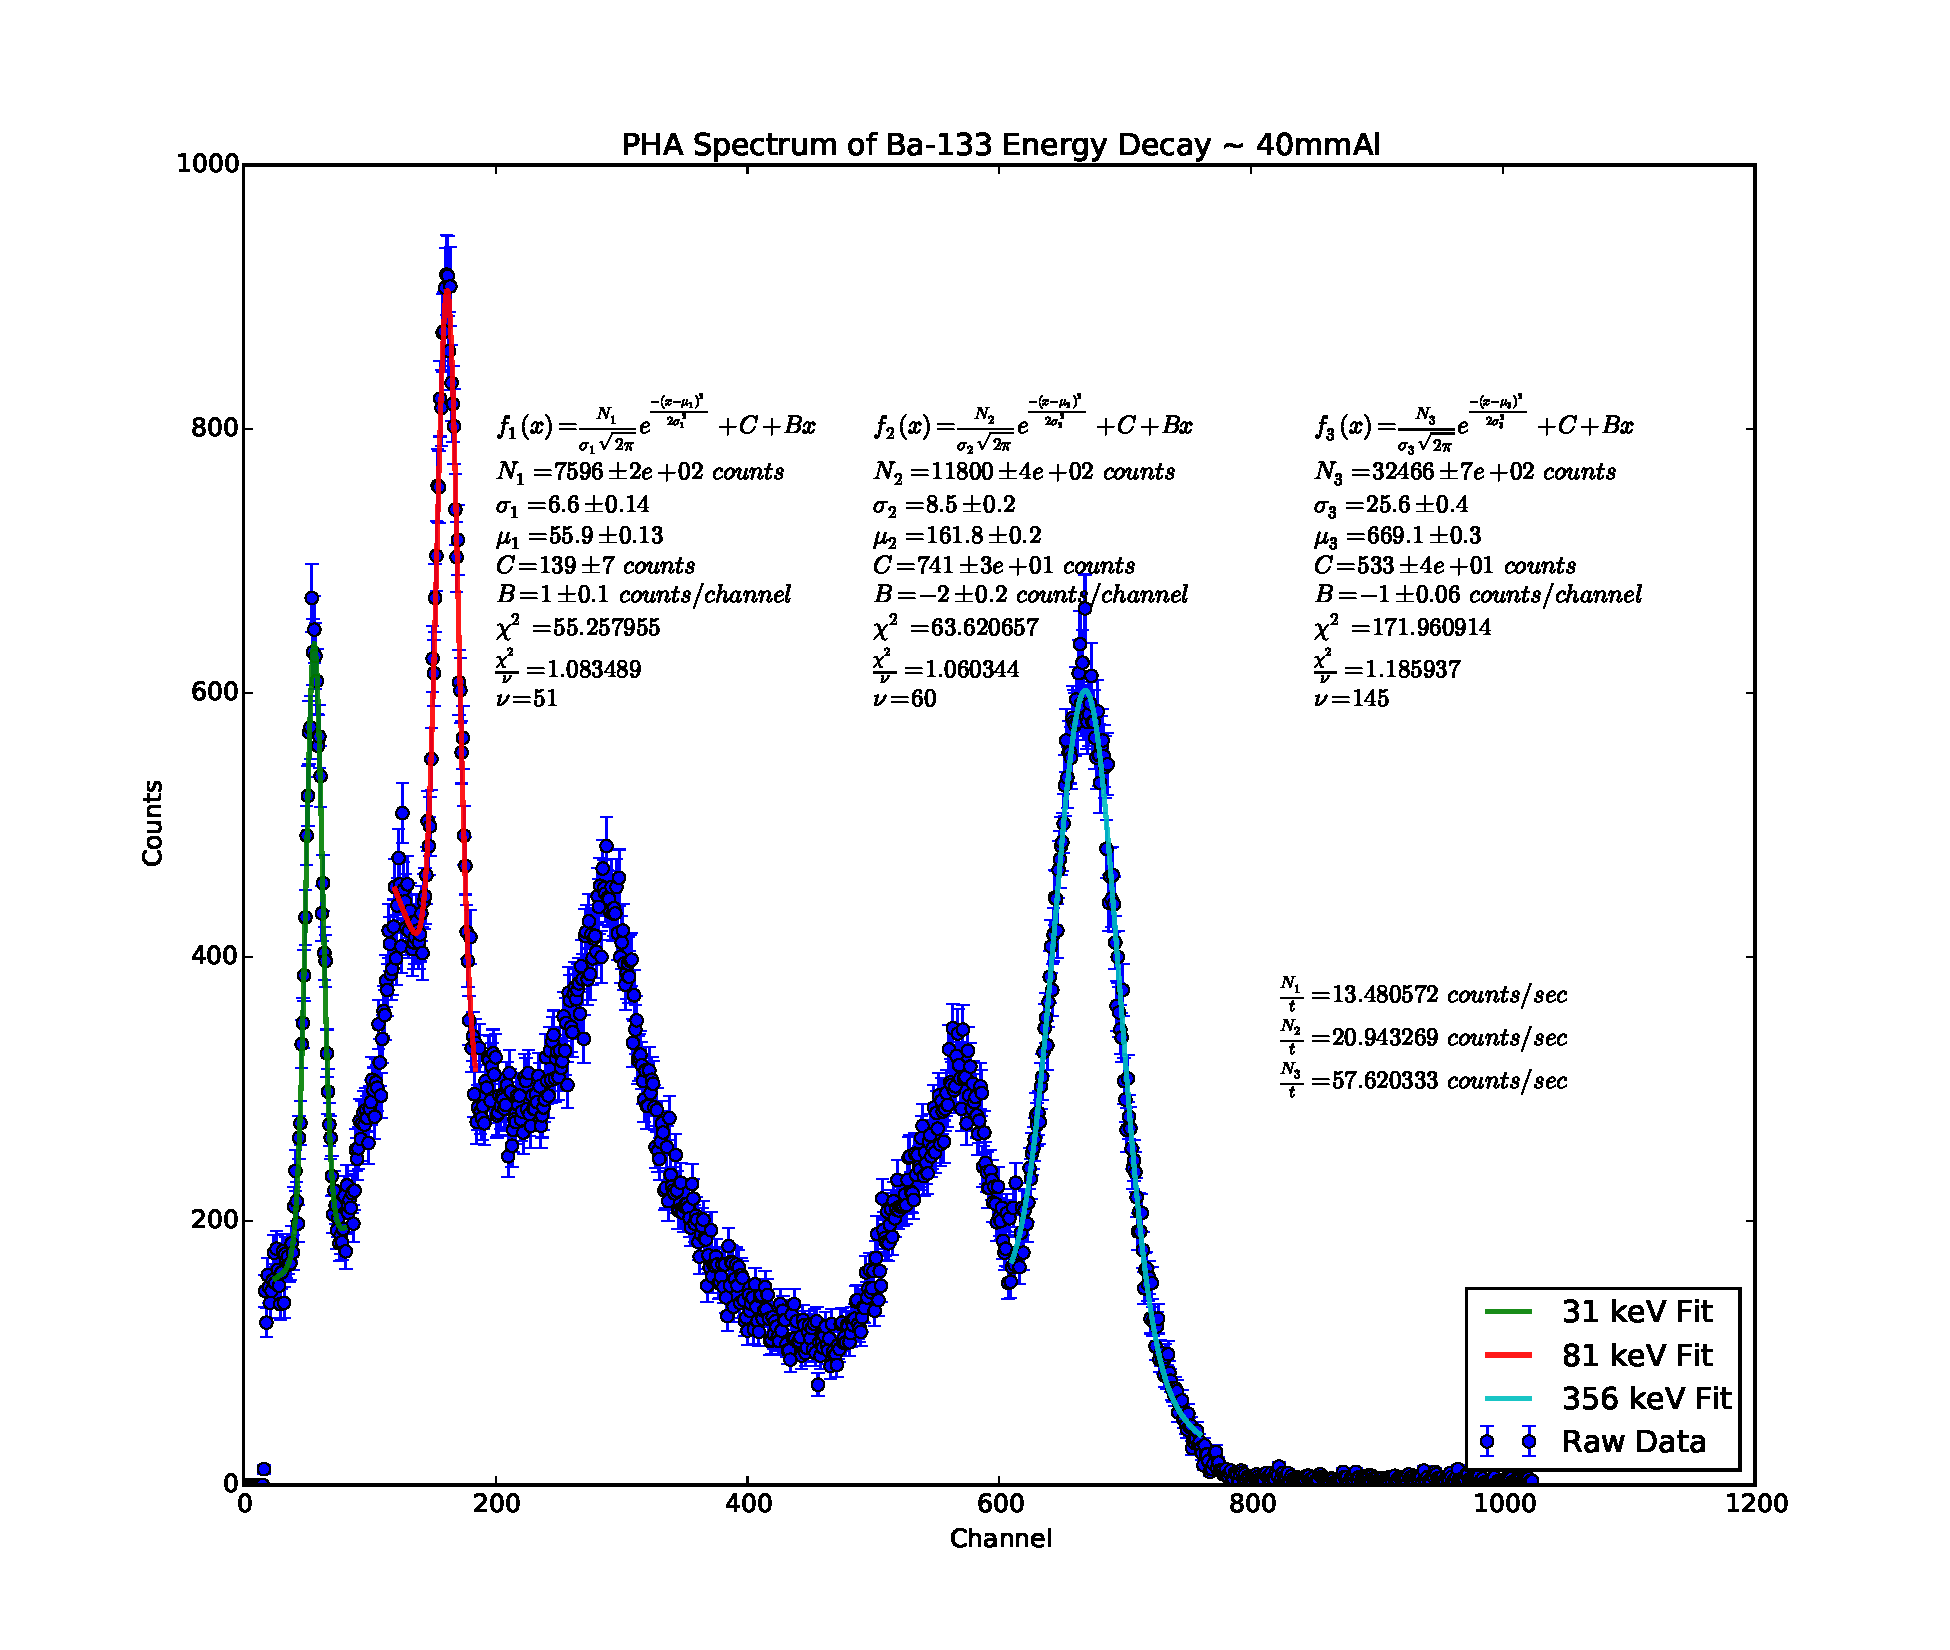
\includegraphics[height=6cm]{../plots/Ba40mmAl.pdf}
		\end{figure}

		An example fit.
	}

	\subsection{Gaussian vs Lorentzian}
	\frame{
		\frametitle{Gaussian vs Lorentzian}	
		Why don't we fit to 
		\begin{equation*}
			L(x) = \frac{1}{\pi} \frac{\frac{1}{2}\Gamma}{(x-x_0)^2 + \frac{1}{2}\Gamma^2} ?
		\end{equation*}

		Because the errors are counting errors - they act on $\bar{x}$ like $\sigma_{\bar{x}}$, the standard deviation of the mean.  And since they are counting errors, they go like $\sqrt{N}$ which is the SDOM.

		They would both fit, but the Gaussian fits better.
	}

	\subsection{Distribution Width}
	\frame{
		\frametitle{Distribution Width}
		\begin{figure}[!htb]
			\centering
			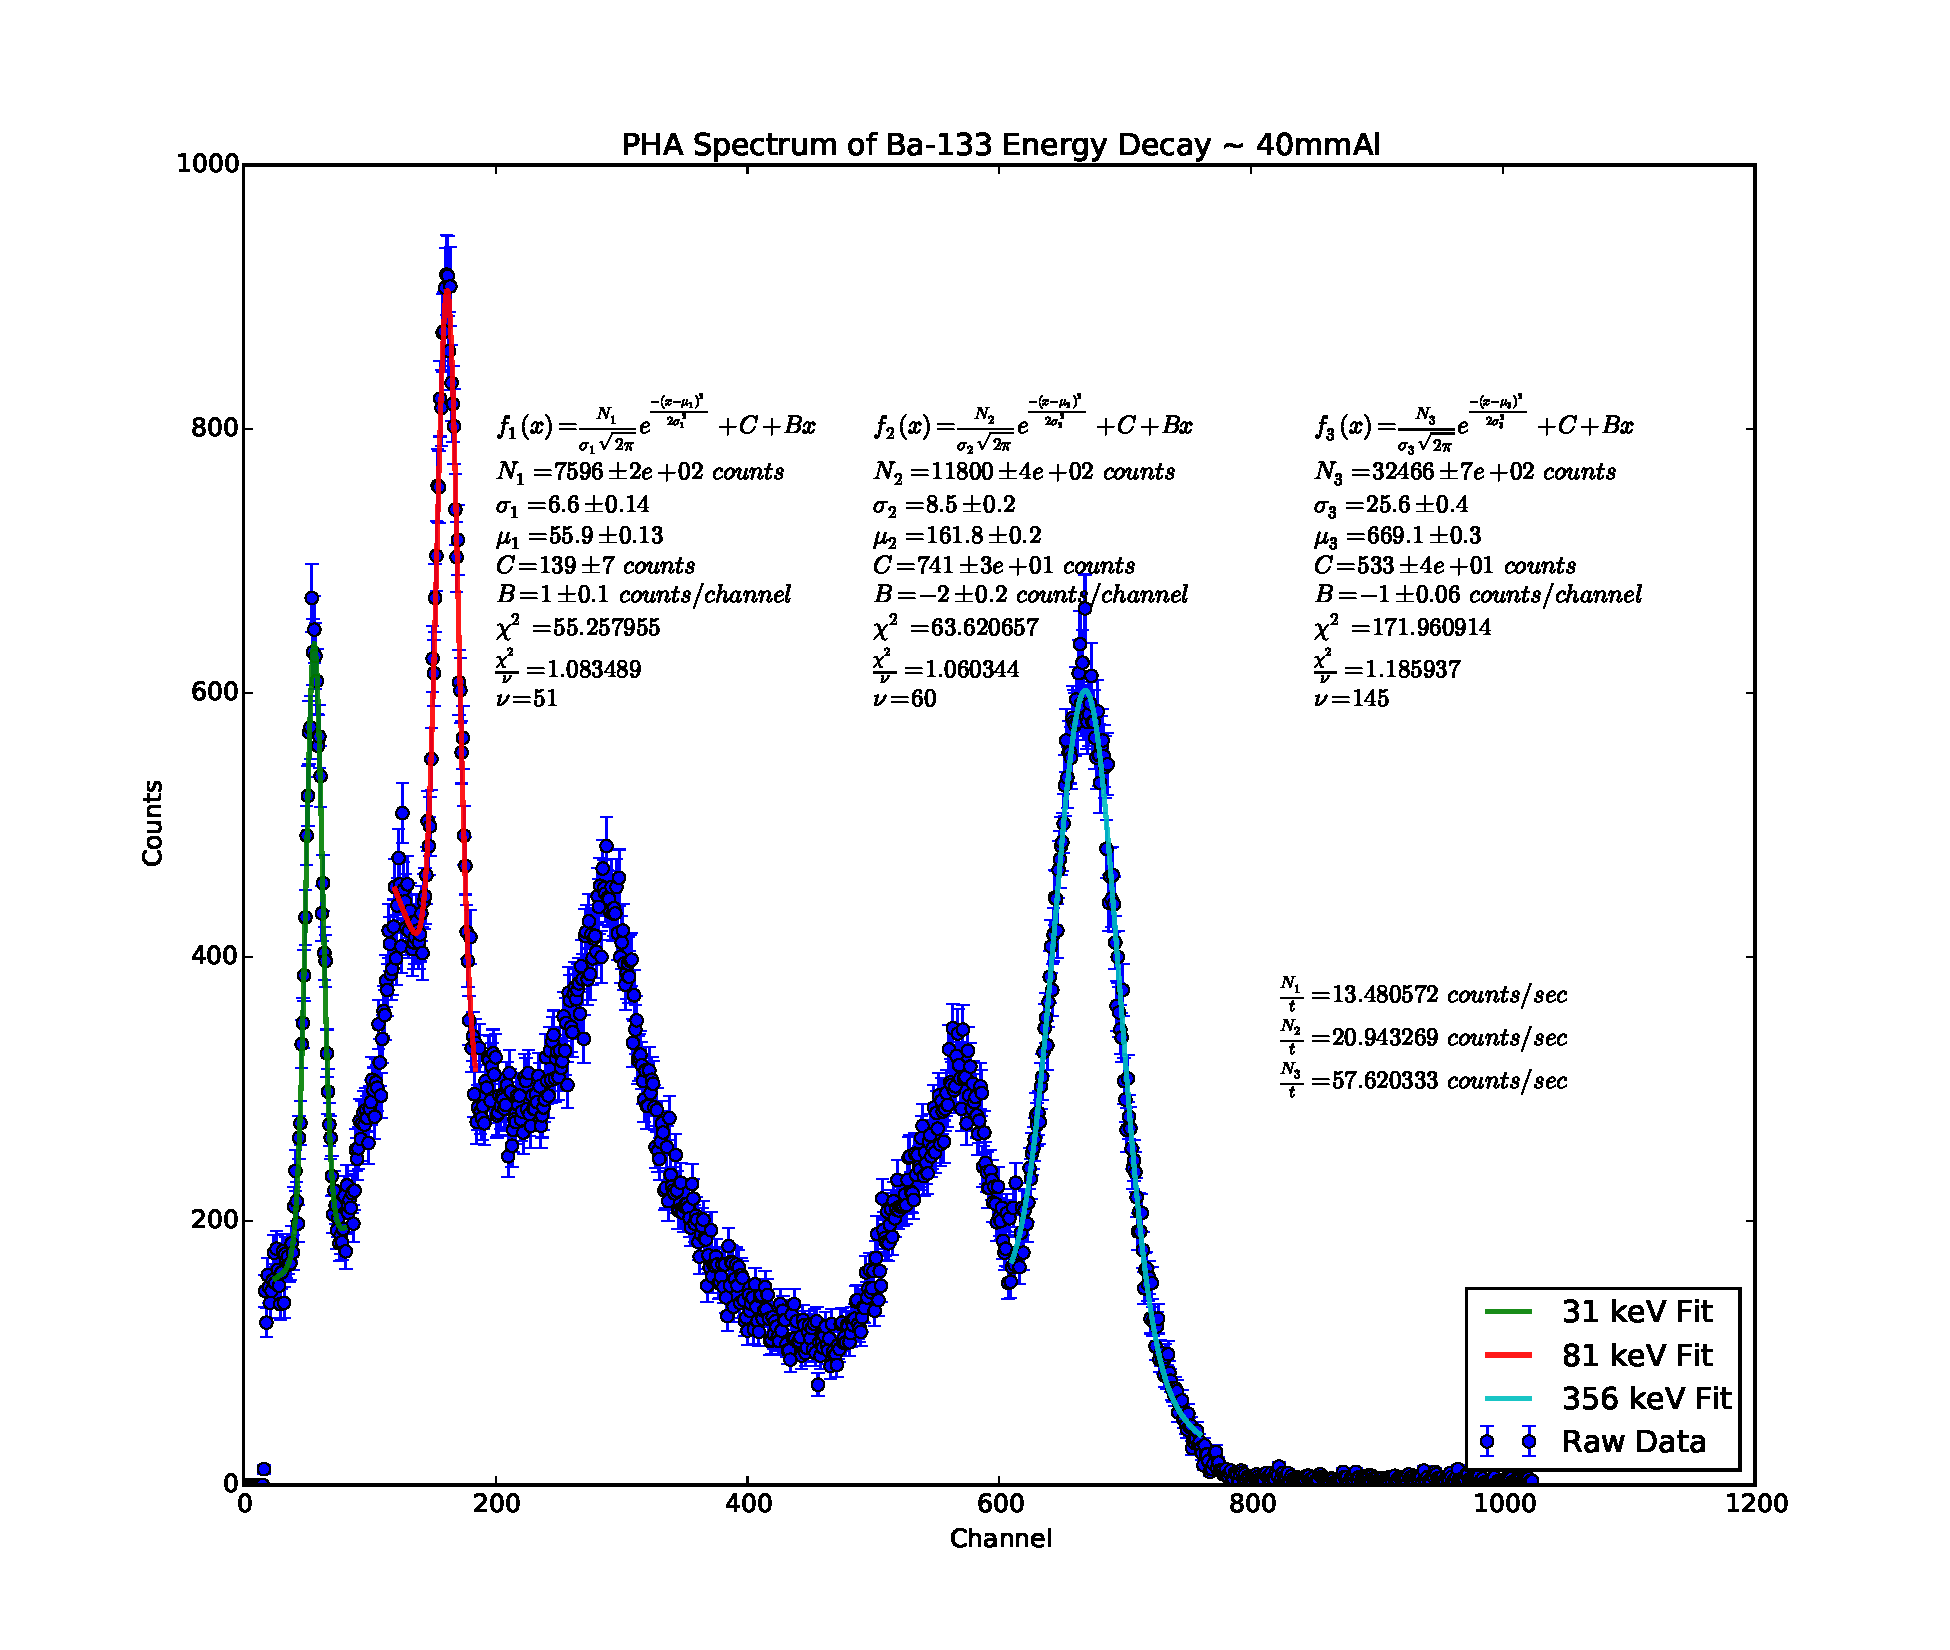
\includegraphics[height=4cm]{../plots/Ba40mmAl.pdf}
		\end{figure}

		The distribution should be a delta function - it isn't because of the detector resolution
	}

	\frame{
		\frametitle{Distribution Width}

		\begin{center}
		\begin{tabular}{|l|l|l|}
			\hline
			Energy (keV) & $\Gamma$ (channels) & $\Gamma/E$\\ \hline \hline
			31 & 8.36 & 26.9\%\\
			81 & 10.18 & 12.6\%\\
			356 & 30.25 & 8.49\%\\ \hline
			511 & 10.68 & 2.09\%\\
			1270 & 16.69 & 1.31\%\\
			\hline
		\end{tabular}
		\end{center}

		Not perfect resolution - this is our $\sigma$ (up to $\Gamma/\sqrt{2}\sqrt{ln(2)}$).
	}

	\subsection{Error Propagation}
	\frame{
		\frametitle{Error Propagation of the PHA fits}
		Since we performed fits, the error of the ith parameter is just:
		\begin{equation*}
			\sigma_{i} = \sqrt{cov(i,i)}
		\end{equation*}

		Because our largest $\delta t$ was less than 0.001\% the uncertainty in parameter i is just $\sigma_{i}$
	}

	\frame{
		\frametitle{Covariance Matrix}
		Scipy and Numpy return the covariance matrix, but here is some information on what it is:
		\begin{gather*}
			X_{i} = (X_i-E(X_i))(X_i-E(X_i))^{T}\\
			\Sigma = \frac{1}{N}\sum_i{X_i}\\
			\Sigma_{ij} \equiv \cov(i,j)
		\end{gather*}
		with each $X_i$ being the squared difference between the datum and the model-estimated parameter - each parameter is expressed as a vector here.
	}

\section{Countrates}
	\subsection{Na}
	\frame{
		\frametitle{Fitting to find $\lambda$}

		We fit to the function 
		\begin{equation*}
			R(x) = R_0e^{-\lambda x} + C
		\end{equation*}
		to extract our values for $\lambda$
	}

	\frame{
		\frametitle{Fitting to find $\lambda$}
		\begin{figure}[!htb]
			\centering
			\includegraphics[height=6cm]{../plots/countrates_na.pdf}
		\end{figure}

		\begin{center}
		\begin{tabular}{|l|l|l|}
			\hline
			Energy & $\lambda$ & $\delta \lambda$\\ \hline
			511 keV & $0.19 \, cm^{-1}$ & $0.03 \, cm^{-1}$\\
			1.27 MeV & $0.09  \, cm^{-1}$ & $0.05 \, cm^{-1}$\\
			\hline
		\end{tabular}
		\end{center}
	}
	\subsection{Ba}
	\frame{
		\frametitle{Fitting to find $\lambda$}

		We fit to the function
		\begin{equation*}
			R(x) = R_0e^{-\lambda x} + R_0'e^{-\tau x} + C
		\end{equation*}
		with $\lambda$ being the compton-like attenuation and $\tau$ being the photoelectric-like attenuation.
	}

	\frame{
		\frametitle{Fitting to find $\lambda$}

		\begin{figure}[!htb]
			\centering
			\includegraphics[height=6cm]{../plots/countrates_ba.pdf}
		\end{figure}

		\begin{center}
		\begin{tabular}{|l|l|l|}
			\hline
			Energy & $\lambda$ & $\delta \lambda$\\ \hline
			31 keV & $2.9 \, cm^{-1}$ & $0.1 \, cm^{-1}$\\
			81 keV & $0.513  \, cm^{-1}$ & $0.06 \, cm^{-1}$\\
			356 keV & $0.24 \, cm^{-1}$ & $0.04 \, cm^{-1}$\\
			\hline
		\end{tabular}
		\end{center}
	}
	\subsection{Comparison to Literature}
	\frame{
		\frametitle{Comparison to Literature}

		\begin{figure}[!htb]
			\centering
			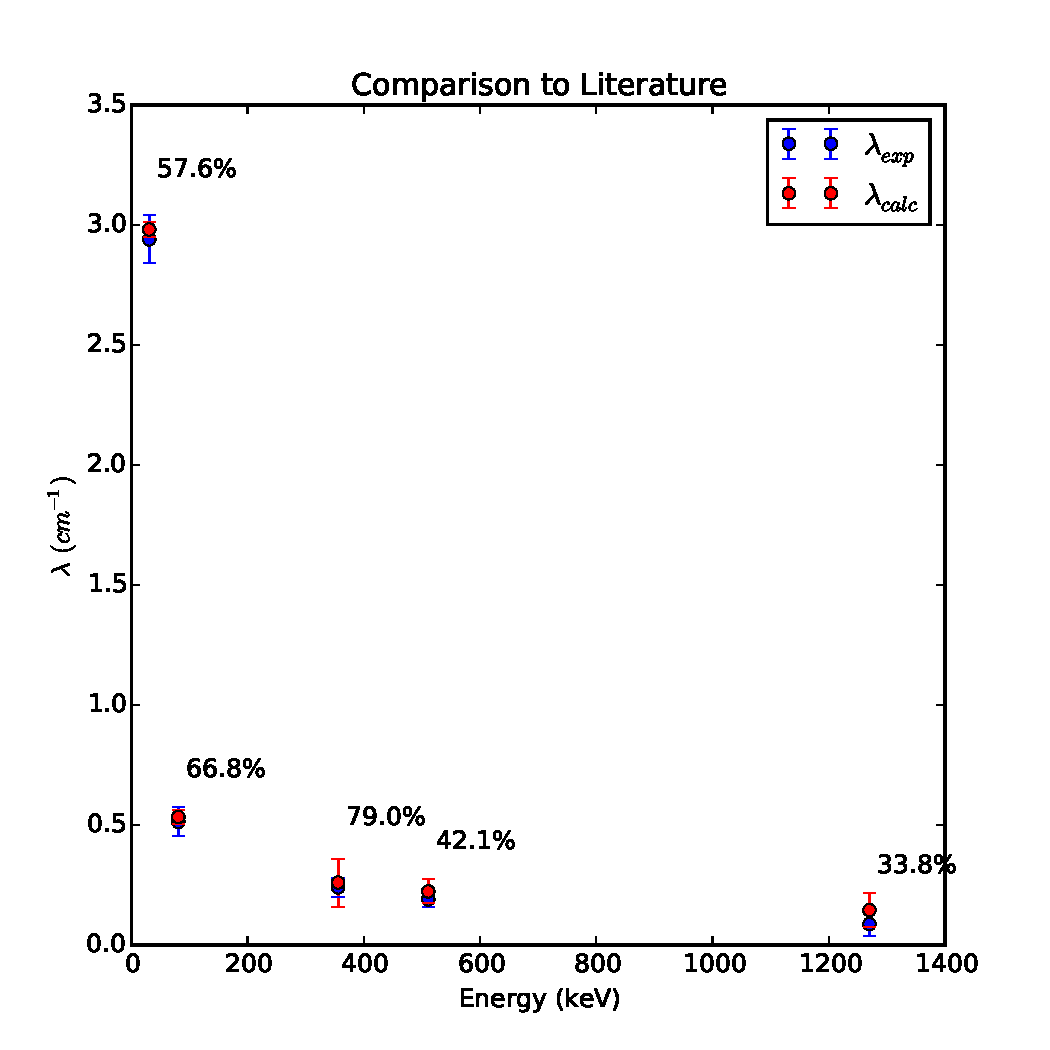
\includegraphics[height=8cm]{../plots/confidence.pdf}
		\end{figure}
	}

	\frame{
		\begin{small}
		\begin{center}
		\begin{tabular}{|l|l|l|l|}
			\hline
			Energy & $\lambda \pm \delta \lambda  \, (cm^{-1})$ & $\lambda_{calc} \pm \delta\lambda_{calc}  (\, cm^{-1})$ & Confidence Level\\ \hline \hline
			31 keV & $2.9 \pm 0.1$ & $2.98 \pm 0.03$ & 57.6\%\\
			81 keV & $0.513 \pm 0.06$ & $0.533 \pm 0.03$ & 66.8\%\\
			356 keV & $0.24 \pm 0.04$ & $0.3 \pm 0.1$ & 79.0\%\\
			511 keV & $0.19 \pm 0.03$ & $0.22 \pm 0.05$ & 42.1\%\\
			1.27 MeV & $0.09 \pm 0.05$ & $0.15 \pm 0.07$ & 33.8\%\\
			\hline
		\end{tabular}
		\end{center}
		\end{small}

		So we have pretty good confidence in our data, I think we did ok.

		The NIST values have uncertainties calculated based on how far the tabulated energy was from our energy and estimating the slope of the area immediately around the point of interest.
	}
	\subsection{Error Propagation}
	\frame{
		\frametitle{Error Propagation of the Countrate Fits}

		We use the same technique as we did with the PHA spectra to calculate the uncertainty in our parameters.  A sample of the data used to calculate the countrates:

		\begin{tiny}
		\begin{center}
		Ba-133 Countrates and Uncertainty\\
		\begin{tabular}{|l|l|l|l|l|l|l|}
			\hline
			Thickness (mm) & N1 (count/s) & N2 (count/s) & N3 (count/s) & $\delta$N1 & $\delta$N2 & $\delta$N3\\ \hline \hline
			56 & 9.044 & 9.910 & 39.361 & 1.915\% & 4.832\% & 1.959\%\\ \hline
			40 & 13.480 & 20.943 & 57.620 & 2.632\% & 3.389\% & 2.156\%\\ \hline
			... & ... & ... & ... & ... & ... & ...\\ \hline
			2 & 303.314 & 145.682 & 156.056 & 1.094\% & 1.302\% & 2.127\%\\ \hline
			1 & 391.492 & 152.985 & 155.885 & 1.032\% & 1.320\% & 2.074\%\\
			\hline
		\end{tabular}
		\end{center}
		\end{tiny}

		Our error bars in the countrate data are exactly the percent error you see above.
	}
	\frame{
		\frametitle{Systematic Uncertainty}
		We noticed that our data (for $\lambda$) was consistently lower than the NIST values, so we tried to fit it and the NIST values to:*
		\begin{equation*}
			f(x) = Ae^{Bx} + Ce^{Dx} + E.
		\end{equation*}
		We found that the difference between our values and the NIST values was in E - it was just an offset.  Furthermore we got a value for E of $0.020\pm0.003$ and so we added that 0.02 to all our uncertainties throughout for $\lambda$.

		\vspace{1cm}

		\tiny{* not shown}
	}


	

\section{References}
	\frame{
		\frametitle{References}
		\begin{thebibliography}{10}
			\setbeamertemplate{bibliography item}[website]
			\bibitem{physics.nist.gov}
				\small{Physics.NIST.gov - Table of XRay Mass Attenuation Coefficients\\
				http://physics.nist.gov/PhysRefData/XrayMassCoef/ElemTab/z13.html}
			\bibitem{lab manual}
				\small{University of Chicago, PHYS 211 Lab Manual - P211 Wiki}

			\setbeamertemplate{bibliography item}[book]
			\bibitem{taylor}
				\small{An Introduction to Error Analysis - John Taylor}
		\end{thebibliography}
	}

\end{document}
